\item \textbf{Walk/non-Walk Classification: Train an HMM model to detect the activity ‘Walk’ using users 1-10 for training. Then, use the model to detect ‘walk’ activity patterns in the data from users 11-15. The goal here is to label during which parts of the data the user were walking. You can adjust the selection criteria by varying the likelihood threshold. Compute the system performance/accuracy across different thresholds (hint: explore ROC curves).}

This question is a learning problem. Figure \ref{fig:pipeline} indicates the pipeline of my solution. For pre-processing part, we used \emph{the re-sampling function} to resize all observations.
\begin{figure}[H]
    \centering
    \begin{minipage}[b]{0.3\textwidth}
        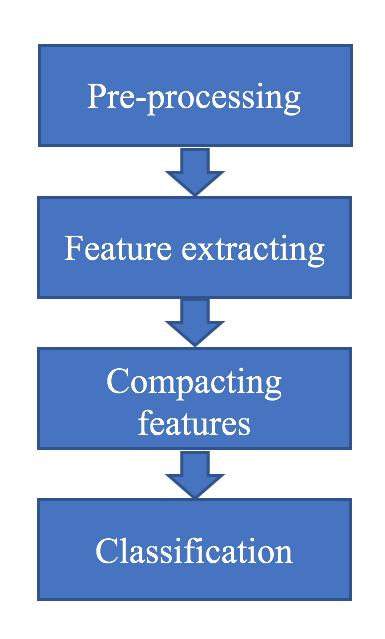
\includegraphics[width=\textwidth]{manuscript/src/figures/Ass3/Ass3_Q2_pipe.png}
    \end{minipage}
    \caption{The pipeline of question 3.}
    \label{fig:pipeline}
\end{figure}

Resizing could delete the effect of zero padding (having the same features for zero values). After that, nine various features were extracted from each observation signal. We also considered a window with the size of 256 samples and an overlap portion of 20 percent. Based on the observation signals, the mean and variance of signal were calculated as features. Also, we found six peak values in the Short-time Fourier transform, with the same algorithm used in the tutorial. Figure \ref{fig:Ass3_Q2_Peak_freq_} shows the peak values for a subset of a signal.


\begin{figure}[H]
    \centering
    \begin{minipage}[b]{1\textwidth}
        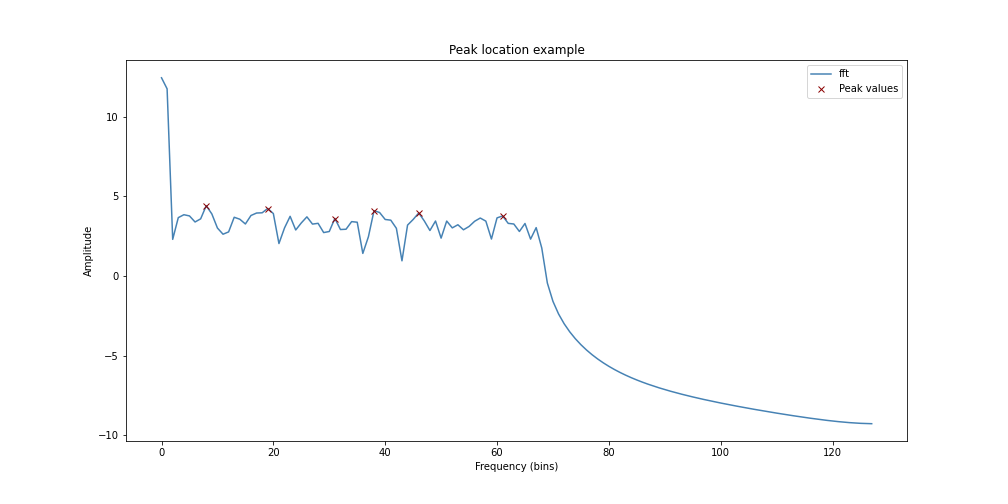
\includegraphics[width=\textwidth]{manuscript/src/figures/Ass3/Ass3_Q2_Peak_freq_.png}
    \end{minipage}
    \caption{The magnitude of STFT and its peak values.}
    \label{fig:Ass3_Q2_Peak_freq_}
\end{figure}


The output of feature extracting is a matrix with dimension of $3 \times 411 \times 9$ for each activity. 
Then features of each observation (x, y, and z) concatenated to each other to produce a matrix of $411 \times 27$ for each user activity. Finally, features were separated based on their activities. The shape of the final array is $15 \times 411 \times 27$; Where 15, 411, and 27 indicate the number of users, windows, and features, respectively.


In the classification part, the array was divided into train and test array. Based on the question, we used users 1 to 10 for training and others for the test. Also, we set the state variable as a loop variable to find the effect of the HMM state in the accuracy.

Because we have only one HMM model trained for walking activity, the output is a probability value. This probability shows whether or not the test features belonged to this activity. To find the best threshold, we used a \emph{for loop}. The results of this model are illustrated below.  


\begin{table}[H]
\centering
\caption{The results of HMM for different states and threshold values.}
\label{tab:Q2_results}
\begin{tabular}{l}
\toprule
    Test accuracy of 2 states HMM for threshold -10000 : $64.29\%$ \\
    Test accuracy of 2 states HMM for threshold -20000 : 57.14\% \\
    Test accuracy of 2 states HMM for threshold -30000 : 57.14\% \\
    Test accuracy of 2 states HMM for threshold -40000 : 50.00\% \\
    Test accuracy of 2 states HMM for threshold -50000 : 50.00\% \\
    Test accuracy of 2 states HMM for threshold -60000 : 71.43\% \\
    Test accuracy of 2 states HMM for threshold -70000 : \textbf{85.71\%}\\
    Test accuracy of 3 states HMM for threshold -10000 : 64.29\% \\
    Test accuracy of 3 states HMM for threshold -20000 : 50.00\% \\
    Test accuracy of 3 states HMM for threshold -30000 : 50.00\% \\
    Test accuracy of 3 states HMM for threshold -40000 : 42.86\% \\
    Test accuracy of 3 states HMM for threshold -50000 : 50.00\% \\
    Test accuracy of 3 states HMM for threshold -60000 : 50.00\% \\
    Test accuracy of 3 states HMM for threshold -70000 : 57.14\% \\
    Test accuracy of 4 states HMM for threshold -10000 : 57.14\% \\
    Test accuracy of 4 states HMM for threshold -20000 : 57.14\% \\
    Test accuracy of 4 states HMM for threshold -30000 : 50.00\% \\
    Test accuracy of 4 states HMM for threshold -40000 : 57.14\% \\
    Test accuracy of 4 states HMM for threshold -50000 : 50.00\% \\
    Test accuracy of 4 states HMM for threshold -60000 : 50.00\% \\
    Test accuracy of 4 states HMM for threshold -70000 : 57.14\% \\
    Test accuracy of 5 states HMM for threshold -10000 : 64.29\% \\
    Test accuracy of 5 states HMM for threshold -20000 : 64.29\% \\
    Test accuracy of 5 states HMM for threshold -30000 : 64.29\% \\
    Test accuracy of 5 states HMM for threshold -40000 : 64.29\% \\
    Test accuracy of 5 states HMM for threshold -50000 : 57.14\% \\
    Test accuracy of 5 states HMM for threshold -60000 : 57.14\% \\
    Test accuracy of 5 states HMM for threshold -70000 : 57.14\% \\
\bottomrule

\end{tabular}
\end{table}

Based on table \ref{tab:Q2_results}, the best result belonged to 2 states HMM with threshold -70000.



 
